\subsection{Revsim: A Reversible Logic Simulator}
  \subsubsection{Overview}
Representing reversible circuits in a way that we could both easily simulate and process them through a genetic algorithm was one of the first challenges we faced. While there have been a number of approaches to reversible circuit synthesis using the genetic algorithm, we found that after conducting a preliminary review, none of them offered the flexibility and extensibility that we were seeking. We set out to develop a software suite capable of simulating any number of reversible circuits while allowing us to manipulate the same circuits at the gate level. In this section, we provide a brief overview and description of the development of our software.

  \subsubsection{Explanation of Simulator Design}
We developed an initial version of our circuit simulator using a functional programming approach but once we had conducted some initial experimentation and testing, it was decided that the code should be refactored to use an object-oriented approach instead. \\

Figure \ref{fig:architecture} shows the basic class structure of the software. Conceptually, a reversible gate has a number of input lines, output lines, 
controls and targets. The abstract {\verb Gate } class formalizes this basic representation of a gate and is subclassed in order to implement arbitrary reversible gates.

Figure \ref{fig:inheritence} shows that there are three main types of gates that we are capable of representing in our framework: ``Single Target'' 
gates such as Toffoli, ``Multiple Target'' gates, like Fredkin and Swap, and ``Same Target'' gates such as inverters, where the target and the control exist on the same line.

The {\verb Cascade } class is used to represent a reversible cascade of gates. It provides the primary functionality for modelling and modifying circuit designs, and is used by other classes such as the {\verb TruthTable } and {\verb GeneticAlgorithm } classes, as described below.

The {\verb TruthTable } class allows us to generate the truth tables of any {\verb Cascade } and compare all or part of the truth table from one circuit with another. Since we must propagate values across each gate in the cascade to generate the output 
values (and since we must do this for all \(2^{n}\) entries in the truth table), the process of generating the truth table is linear in the 
number of gates of the circuit and exponential in the number of variables ($\mathcal{O}(2^{mn})$, where $m$ is the number of gates in the cascade, and $n$ is the number of variable lines).

\pagebreak
\begin{figure}[H]
\centering
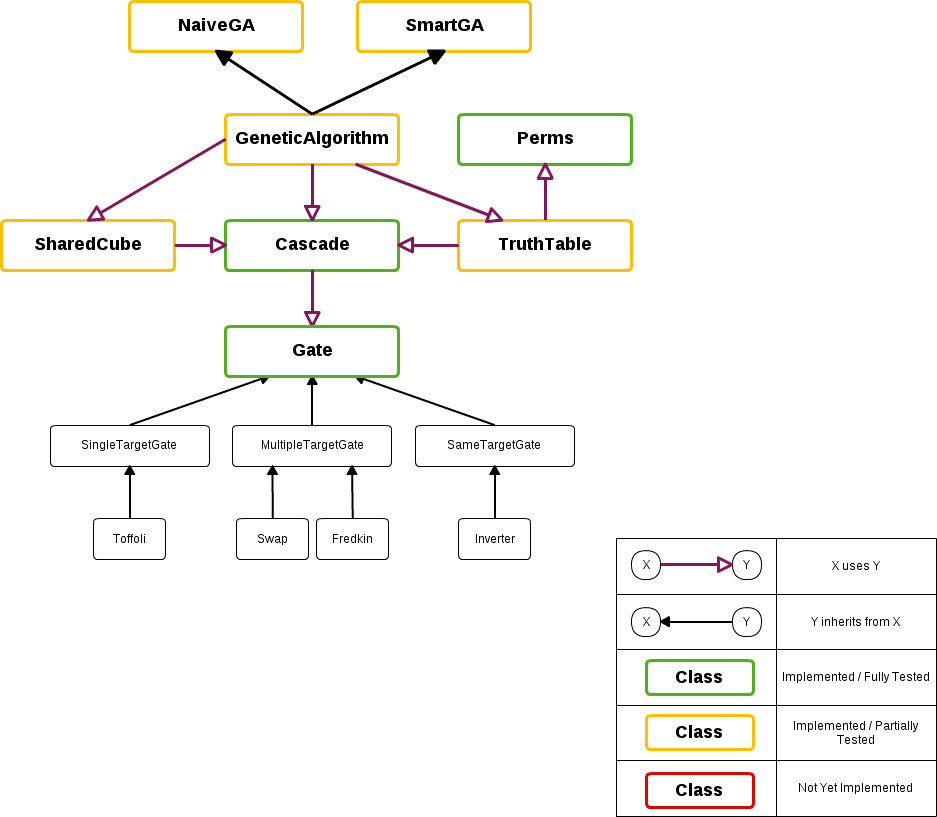
\includegraphics[width=130mm]{diagrams/architecture.png}
\caption{Class structure of Revsim}
\label{fig:architecture}
\end{figure}


\begin{figure}[H]
\centering
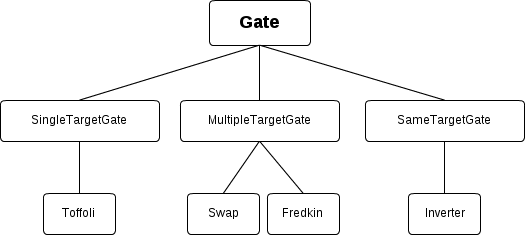
\includegraphics[width=120mm]{diagrams/gate_inheritence.png}
\caption{Gate inheritence in Revsim}
\label{fig:inheritence}
\end{figure}

\pagebreak

Our simulation software also has a number of classes that provide additional extensibility. For example there are input/output 
classes that allow us to directly read from and write to files in the \url{www.revlib.org}'s {\verb *.real } file format. Our initial genetic algorithm implementation 
required us to manually enter each goal cascade that we wanted to test against, but using these helper classes we were able to 
implement the ability to parse any .real file and use its target output function in the fitness calculations for our genetic 
algorithm. We also developed an experimental {\verb SharedCube } class that allows us to generate and use the shared cube 
representation that we were initially going to use to represent individuals in our genetic algorithm so that we could apply a 
number of the rule based transformations from \cite{Nayeem2011} but after implementing it, we decided 
on using the representation described below. Due to time constraints, this was not implemented in the Release Master of the software.

  \subsubsection{Description of Our Genetic Algorithm}

\paragraph{Representation} 

We initially explored using a shared cube representation for the individuals in used in our algorithm however while we initially 
thought that the transformational rules  in \cite{Thornton2007} would be useful in implementing mutation, we found it difficult to implement 
in the context of our genetic algorithm and we were not able to discover an appropriate method of implementing crossover using the shared 
cube representation. Instead. we settled on using the cascade representation from our Cascade class which stores the list of gates used 
in the circuit for the individuals in our populations.

Our algorithm initially reads in a circuit that specifies the desired output behaviour and then creates the initial population as copies 
of the initial circuit that have been mutated from the initial circuit up to a maximum number of mutations specified in the initial 
conditions. Once the initial population is generated, the cycle of fitness evaluations, selection, mutation and crossover repeats until 
one of two terminal conditions are reached, either a fitness of 1.0 or a maximum number of generations.

\paragraph{Fitness and Selection} 

Our fitness metric measured how closely the truth table of the current individual matched the truth table of the of 
the desired output behaviour. It basically performs an exhaustive comparison and so the number of comparisons needed are approximately
 exponential in the number of variables (linewidth) of the circuit.  


\paragraph{Crossover}

Our implementation of crossover selects the best two individuals as parents and creates two child individuals. The first child has the 
first half of the gates from parent 1 and the second half from parent 2 while the second child has the first half of the gates from 
parent 2 and the second half from parent 1. The children are then added to the population for the next iteration of the algorithm. 

\paragraph{Mutation}

The mutation function randomly selects a certain number of gates and will either replace or remove them from the cascade of the 
individuals it is being applied to.

%\paragraph{Parameter Variations.}

%Our initial parameters

\paragraph{Parallelization in Revsim} 

\begin{figure}
  \begin{center}
    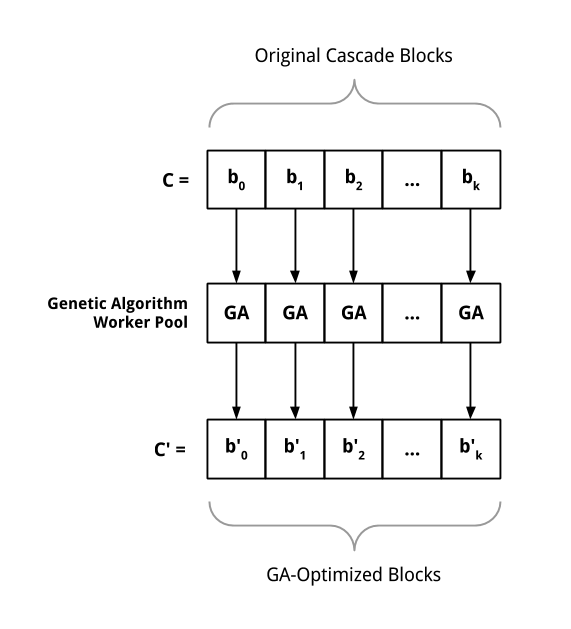
\includegraphics[width=100mm]{diagrams/parallelization.png}
  \end{center}
  \caption{Parallelization in Revsim.}
  \label{fig:parallel}
\end{figure}

In order to efficiently optimize large cascades on multi-processing systems, Revsim uses a ``splitting'' approach, wherein cascades are partitioned into sub-cascade ``blocks'', which are then optimized independently. Each block is passed through a corresponding instance of the Genetic Algorithm class, which runs in a Python sub-process. The host operating system is then free to delegate the sub-process to a particular processing unit, which allows the system to process many blocks in parallel. This process is illustrated in Figure \ref{fig:parallel}. \\

Once a genetic algorithm sub-process completes, the resulting (optimized) cascade is returned to the main Python thread which delegates further blocks to genetic algorithm sub-processes. These steps are continued until there are no unoptimized blocks remaining in the cascade. \\

Since Revsim's genetic algorithm class preserves all function outputs when performing optimizations, we can show that each input block is logically equivalent to output blocks. If a particular block cannot be optimized (in the case when the maximum generation count is exceeded), then the unoptimized block is returned.


\paragraph{Avoiding Global Interpreter Lock} When using an interpreted programming language such as Python, it is important to keep in mind that if each thread is running in the same interpreter instance, it is possible that one thread may ``lock'' the interpreter, preventing the execution of other threads. Thus, rather than using threads, Revsim uses \emph{sub-processes} in order to delegate tasks to separate processing units. Each sub-process runs its own interpreter instance, thus sidestepping Global Interpreter Lock. This advantage comes at the cost of increased interpreter overhead, but this cost is negligible when the benefits of sub-processing are considered. 

\paragraph{Grid Computing}

We first spent some time adapting our software so that it could be run across the University of Lethbridge's HTCondor computing grid. 
Because we needed to test a number of circuits across a set of variable initial parameters one of the key challenges we faced was 
automating the task of creating the HTCondor job submissions. We were able to script a solution that allows us to automatically take 
a batch of any number reversible circuits in .real format and output a set of submission-ready executables that we could run across 
the HTCondor grid. This provided a significant increase in the speed we were able to generate tests and obtain results.
